% Le damos al documento formato de artítulo, con letra tamaño 12pt e idioma español
\documentclass[12pt, spanish]{article}


%%%%%% IDIOMA Y FUENTES
% Algunos comandos pa. a configurar documentos en idioma español
% Más info: overleaf.com/learn/latex/International_language_support

% El paquete T1 es para que la separación de palabras entre renglones funcione bien (para español o idiomas con acentos o caracteres especiales)
\usepackage[T1]{fontenc}
% Para soportar el formato español (por ejemplo, cambia la palabra clave "Theorem" por "Teorema")
% "es-noindentfirst" sirve para no indentar los primeros párrafos de cada sección
% "es-noindentfirst" sirve para no indentar los primeros párrafos de cada sección
% "shorthands=off" quita algunos shortcuts confusos para tipear comillas (por ej. << >>)
\usepackage[spanish, es-noindentfirst, shorthands=off]{babel}
% Configura las dimensiones de la página y márgenes
\usepackage[a4paper,width=150mm,top=25mm,bottom=25mm]{geometry}
% Encabezados
\usepackage{fancyhdr}
\pagestyle{fancy} % Usamos el estilo fancy
% Para personalizar pie de página
% \fancyfoot{} % se borra el estilo actual
% % Para agregar una línea en el pie de página
% \renewcommand{\footrulewidth}{0.4pt}
% % Para agregar la página a la derecha
% \fancyfoot[R]{\thepage}
% % Para calmar una warning del paquete fancyhdr cuando hay títulos largos
\setlength{\headheight}{14.61858pt}


% Para evitar warnings molestas sobre líneas que hacen un poco de overflow en un renglón
\emergencystretch=1em

% % Para customizar en profundidad las secciones y capítulos
% \usepackage{titlesec}
% % Modificamos el formato de los capítulos
% \titleformat{\part} % comando
% [display] % forma
% {\vspace{1cm}\bfseries\LARGE\raggedright} % formato
% {Parte\ \thepart} % label
% {2ex} % separación
% {\huge} % a ejecutar antes del título
% [\hrule] % a ejecutar después del título - \hrule dibuja una línea

% % Agregamos la parte en la izquierda del encabezado
% \fancyhead[L]{\thepart. \partmark}

%%%%%% SIMBOLOS y FUENTES
\usepackage{amsmath}
\usepackage{amsthm}
\usepackage{amssymb}
% Para que anden juntas mathcal y mathscr (dos fuentes de math mode)
\usepackage[scr=rsfs]{mathalpha}


%%%%%% FORMATO GENERAL
% Para escribir con colores
\usepackage{xcolor}
% Para usar comillas con el comando \say{} 
\usepackage{dirtytalk}
% Para mejor subrayado
\usepackage{ulem}
% Para resaltar sintaxis de código
% Si vas a correr este paquete localmente, tenés que instalar Pygments.
% minted te puede luchar un poco, yo logré correrlo en VS Code compilando con pdflatex
% y agregándole la flag -shell-escape al compilador
\usepackage{minted}
\usemintedstyle{friendly}
\definecolor{light_gray}{gray}{0.9} % color para el background del código
% Para citas con autor
\usepackage{epigraph}
% Para calmar algunas warnings sobre el paquete babel y minted
\usepackage{csquotes}
% Para configurar formato de los links
\usepackage{hyperref}
\hypersetup{
    colorlinks=true, % colorea links en lugar de recuadrarlos
    linktoc=all, % hace que el índice contenga links a las secciones
    linkcolor=black, % color de los links
    allcolors=black, % ...no recuerdo pero lo dejamos
}
% Para incluir tipo del resultado en cada cita usando \cref (en lugar de \ref)
\usepackage[nameinlink]{cleveref}
% Para configurar formato de listas
% \itemsep = vertical space added after each item in the list.
% \parsep = vertical space added after each paragraph in the list.
% \topsep = vertical space added above and below the list.
% \partopsep = vertical space added above and below the list, but only if the list starts a new paragraph.
\usepackage{enumitem}
\setlist[enumerate]{
    topsep=0.17cm,
    itemsep=0.1cm,
    parsep=0.05cm,
}
\setlist[itemize]{
    topsep=0.17cm,
    itemsep=0.1cm,
    parsep=0.05cm,
    % label=$\bullet$ % Para cambiar la label para todos los itemize
}
\renewcommand\labelitemi{\labelitemfont \textbullet}
\renewcommand\labelitemii {\labelitemfont \bfseries \textendash}
% Más niveles de personalización
% \renewcommand\labelitemiii{\labelitemfont \textasteriskcentered}
% \renewcommand\labelitemiv{ \labelitemfont \textperiodcentered}

% Para agregar cajas de texto lindas
\usepackage{tcolorbox}
% Para generar texto dummy para rellenar texto en algunos lugares
\usepackage{lipsum}


%%%%%% GRAFICOS E IMAGENES
% Para generar cualquier gráficos que te imagines
\usepackage{tikz}
% Para generar diagramas conmutativos
\usepackage{tikz-cd}
% Para grafos
\usetikzlibrary{graphs}
% Para la forma alternativa de mostrar grafos
\tikzset{
    point/.style = {circle, draw, inner sep=0.04cm,fill,node contents={}},
}
% Para evitar problemas en tikz con acentos en español
\usetikzlibrary{babel}
% Paquete alternativo para gráficos de funciones
\usepackage{pgfplots}
\pgfplotsset{compat=1.18} % Compatibilidad de versiones del paquete
% Para crear tablas de archivos .csv
\usepackage{csvsimple}
% Para agregar imágenes
\usepackage{graphicx}
% Para wrappear imágenes en texto
\usepackage{wrapfig}
\setlength{\intextsep}{.2cm} % configuramos márgenes 
\setlength{\columnsep}{.2cm} % configuramos márgenes 
% Para formatear interlineado
\usepackage{setspace}




%%%%%% BIBLIOGRAFIA
% Más info: overleaf.com/learn/latex/Bibliography_management_in_LaTeX
% Más info sobre estilos: overleaf.com/learn/latex/Biblatex_bibliography_styles
\usepackage[
    backend=biber, % compilador
    style=alphabetic, % la referencia tiene letras en vez de números ('numeric' para números)
    sorting=anyt % ordenamiento de las referencias
]{biblatex}
% Linkeamos el archivo con las referencias
\addbibresource{bibliografia/bibliografia.bib}


%%%%%% TEOREMAS Y ENTORNOS
% Especificamos el nombre del entorno
\providecommand{\definitionname}{Definición}
% Comandos para definir entornos de definiciones, teoremas, etc.
\theoremstyle{definition} % estilo de lo que se va a definir
% Con \newtheorem se pueden definir entornos para teoremas, definiciones, etc. El primer argumento es el nombre del entorno (en este caso defn) y el segundo es el texto que aparece cuando se usa el entorno (en este caso dejamos que LaTeX lo busque, deberia ser "Definición").
% Más info: overleaf.com/learn/latex/Theorems_and_proofs
\newtheorem{defn}{\protect\definitionname}

\providecommand{\remarkname}{Observación}
\theoremstyle{remark} % observación
\newtheorem{rem}[defn]{\protect\remarkname}

\providecommand{\theoremname}{Teorema}
\theoremstyle{plain} % teorema
\newtheorem{thm}[defn]{\protect\theoremname}

\providecommand{\corollaryname}{Corolario}
\theoremstyle{plain} % corolario
\newtheorem{cor}[defn]{\protect\corollaryname}

\providecommand{\lemmaname}{Lema}
\theoremstyle{plain} % lema
\newtheorem{lem}[defn]{\protect\lemmaname}

\providecommand{\propositionname}{Proposición}
\theoremstyle{plain} % proposición
\newtheorem{prop}[defn]{\protect\propositionname}

\providecommand{\conjecturename}{Conjetura}
\theoremstyle{plain} % conjetura
\newtheorem*{conjecture}{\protect\conjecturename}

\providecommand{\examplename}{Ejemplo}
\theoremstyle{remark} % ejemplo
\newtheorem{example}[defn]{\protect\examplename}

% Definimos un entorno para demostraciones
\newenvironment{dem}{\noindent\textit{Demostración.}}{\hfill\qed\par\vspace{10pt}}

% Este otro entorno nos permite reemplazar el texto "Demostración" al principio del comando \dem por otro texto.
% Ejemplo:
% \begin{demcustom}{Demostración de la primera parte del \cref{teorema:algun teorema referenciado aca}}
%   ... [contenido acá] ...
% \end{demcustom}
\newenvironment{demcustom}[1]{\noindent\textit{#1.}}{\hfill\qed\par\vspace{10pt}}


%%%%%% COMANDOS MISCELANEOS
% Algunos comandos útiles para agilizar el tipeo
\newcommand{\real}[0]{\mathbb{R}} % números reales
\newcommand{\nat}[0]{\mathbb{N}} % números naturales
\newcommand{\id}[0]{\mathrm{id}} % función identidad
\newcommand{\spanev}[0]{\mathrm{span}} % espacio vectorial generado
\newcommand{\sgn}[0]{\mathrm{sgn}} % función signo
\newcommand{\re}[1]{Re(#1)} % parte real de un número complejo
\newcommand{\im}[1]{Im(#1)} % parte imaginaria de un número complejo
\newcommand{\rest}[2]{{#1}_{|_{#2}}} % Restricción de una función a un conjunto
\newcommand{\norm}[1]{\|#1\|} % norma
\newcommand{\prodint}[2]{\langle #1, #2 \rangle} % producto escalar

% Para probar implicancias en teoremas con equivalencias
\newcommand{\implicancia}[2]{\vspace{0.4em}\noindent$\text{\textit{(#1)}}\hspace{-0.4em}\implies\hspace{-0.4em}\text{\textit{(#2)}}$}

% "Tal que" en definiciones de conjuntos por comprensión
% Ejemplo: A = \{ x\in\real \sep x > 0 \} 
\newcommand{\sep}[0]{\,:\,}

% Así se definen comandos que permiten tener subíndices "abajo"
\DeclareMathOperator*{\supess}{sup\,ess}
\DeclareMathOperator*{\infess}{inf\,ess}

% Se pueden definir colores en LaTeX!
\definecolor{salmon}{HTML}{c23d52} % purplish gray

%%%%%% TITULO DEL DOCUMENTO
\title{Taller de \LaTeX}
\author{Matías Palumbo}
% Por defecto la fecha del artículo es \today (fecha de hoy). Se puede personalizar
\date{24 de septiembre de 2024}



\begin{document}

% Agrega el título/autor/fecha especificado antes
\maketitle

% Mostramos el índice
\tableofcontents

% Salto de página
\pagebreak

\section{Recursos generales}
\noindent Algunos recursos útiles:
\begin{enumerate}
    \item \href{www.overleaf.com}{overleaf.com} $\to$ la biblia de \LaTeX
    \item \href{www.manualdelatex.com}{manualdelatex.com} $\to$ muchos comandos para símbolos y tutoriales útiles
    \item \href{www.drive.google.com/drive/folders/1OXJNANEtlrzC934mgEcmJNUbtBfR32l9?usp=drive_link}{Google Drive del taller!}
    \item \href{https://ctan.org/?lang=en}{The Comprehensive TeX Archive Network (CTAN)}
    \item \href{https://manualdelatex.com/}{manualdelatex.com} $\to$ listas de símbolos y tutoriales
\end{enumerate}



\section{Estructura de un documento}

Acá estamos dentro de una sección (sección \thesection).

\subsection{Subsecciones}

Esto está dentro de una subsección (subsección \thesubsection).

\subsubsection{Sub-subsecciones}

Podemos llegar hasta sub-subsecciones (sub-subsección \thesubsubsection).

\subsection*{Subsecciones no numeradas}

Las secciones/subsecciones/etc. pueden no estar numeradas.


\section{Ecuaciones}

Hay varias formas distintas de incluir ecuaciones en \LaTeX. Las ecuaciones pueden estar en línea con el texto ($f(x) = e^{-x}$) o estar en bloque: 
\[
(x+y)^n = \sum_{k=0}^n \binom{n}{k} x^k y^{n-k}.
\]
Las ecuaciones en línea (\textit{inline}) intentan ocupar menos espacio vertical, por lo que algunos operadores muestran los subíndices al costado en lugar de debajo del operador: $\sum_{k=0}^n$. Para incluir los subíndices debajo del operador en estas ecuaciones se puede usar el comando \verb|\limits|: $\sum\limits_{k=0}^n$. El comando \verb|\nolimits| hace lo contrario:
\[
(x+y)^n = \sum\nolimits_{k=0}^n \binom{n}{k} x^k y^{n-k}.
\]

Las ecuaciones en bloque también pueden agregarse con el entorno \verb|equation| (numeradas) o \verb|equation*| (no numeradas):
\begin{equation}
    \text{erf}(x) = \frac{2}{\sqrt{\pi}} \int_0^x e^{-t^2} dt.
\end{equation}

El tamaño de paréntesis, llaves, etc., puede especificarse (todos los tamaños \href{www.overleaf.com/learn/latex/Brackets_and_Parentheses}{acá}): \[
    (\frac{y}{z})^x\;\;\;\;\;\Big(\frac{y}{z}\Big)^x.
\]
Los comandos \verb|\left| y \verb|\right| permiten automatizar este proceso:
\[
    \left(\frac{y}{z}\right)^x = \left[ a(0) + \int_0^\infty f(t)dt\right] + \left. \frac{x^{n+1}}{n+1} \right|_0^\infty.
\]

Para cadenas largas de igualdades, puede ser útil el entorno \verb|align| (o \verb|align*| para no numerar). El símbolo \verb|&| se usa para alinear las diferentes ecuaciones, y se usa \verb|\\| para cambiar de línea.
\begin{align*}
    \frac{p_n(x - y)}{1 + p_n(x - y)} &\leq \frac{p_n(x - z) + p_n(z - y)}{1 + p_n(x - z) + p_n(z - y)} \\
    &= \frac{p_n(x - z)}{1 + p_n(x - z) + p_n(z - y)} + \frac{p_n(z - y)}{1 + p_n(x - z) + p_n(z - y)} \\
    &\leq \frac{p_n(x - z)}{1 + p_n(x - z)} + \frac{p_n(z - y)}{1 + p_n(z - y)}.
\end{align*}

Otros entornos útiles son:
\begin{itemize}
    \item \textit{Matrices} (más info \href{www.overleaf.com/learn/latex/Matrices}{acá}):
    \[
        \begin{pmatrix}
        a & b & c\\
        d & e & f
        \end{pmatrix}\hspace{1.5cm}
        \begin{vmatrix}
        \sin\theta & \cos\theta\\
        \cos\varphi & -\sin\varphi
        \end{vmatrix}
    \]
    \item \textit{Arreglos} (parecidos a las matrices, más personalizables). La justificación de los elementos de cada columna del arreglo se controla con las llaves que hay justo tras \verb|\begin{array}|. Las opciones son \verb|r| (derecha) y cambiarlo por \verb|c| (centrado) o \verb|l| (izquierda).
    \[
      \begin{array}{cc}
        \alpha & \beta \\
         \gamma & \delta
      \end{array}\hspace{1.5cm}
      \begin{array}{c||cc|r}
        -1 & 2 &  3 &   0 \\
         3 & 4 & -7 &   2\\
         6 & 5 & 90 & -11
      \end{array}
    \]
    \item \textit{Funciones por casos}:
    \[
        \sgn(x) = \begin{cases}
            1& \text{si $x > 0$},\\
            -1& \text{si $x < 0$}.
        \end{cases}
    \]
\end{itemize}




\section{Formato de texto}
\noindent Algunos tips sobre formato:
\begin{itemize}
    \item Para tipear comillas: ``nativamente'' o \say{con el comando \textbackslash say}.
    \item Subrayado con el comando \underline{underline} versus con el paquete \uline{ulem}. El paquete ulem tiene más opciones de subrayado, estas son algunas sacadas de las docs:
    \begin{itemize}
        \item \uuline{urgent}: double-underlined text 
        \item \uwave{boat}: wavy underline
        \item \sout{wrong}: line struck through word
        \item \xout{removed}: marked over
        \item \dashuline{dashing}: dashed underline
        \item \dotuline{dotty}: dotted underline
    \end{itemize}
    \item Para fuente monoespaciada: el comando \verb|verb|.
    \item Para citas y frases importantes:
        \begin{quote}
            The major problem—one of the major problems, for there are several—one of the many major problems with governing people is that of whom you get to do it; or rather of who manages to get people to let them do it to them. To summarize: it is a well-known fact that those people who most want to rule people are, ipso facto, those least suited to do it. To summarize the summary: anyone who is capable of getting themselves made President should on no account be allowed to do the job.
            \begin{flushright}
                \textit{Douglas Adams, The Hitchhiker’s Guide to the Galaxy}
            \end{flushright}
        \end{quote}

    \item Para resaltar sintaxis de código se puede usar el paquete \verb|minted|. Más info \href{https://www.overleaf.com/learn/latex/Code_Highlighting_with_minted}{acá}.
    \begin{minted}[
        baselinestretch=1.2, % espacio entre líneas
        bgcolor=light_gray,
        fontsize=\footnotesize,
        linenos, % incluye numeros de lineas
    ]
    {python}
def pick_random_color():
    hexs = [random.choice('ABCDEF0123456789') for _ in range(6)]
    return '#' + ''.join(hexs)
    \end{minted}    
    \item Se puede \textcolor{cyan}{escribir} en \textcolor{salmon}{\underline{colores}} con el paquete \verb|xcolor| y el comando \verb|\textcolor|.
    \item Se pueden trazar líneas para separar partes del documento con el comando \verb|\hrule|.

\end{itemize}

\section{Teoremas y otras formas de encapsular texto}

\subsection{Entornos de teoremas}

Se puede especificar el nombre/autor del teorema/definición/etc. entre corchetes:
\[
    \verb|\begin{thm}[...]|
\]

\begin{thm}[Primer Teorema Fundamental del Cálculo]
    Sea $f:[a, b]\to\real$ una función continua, y sea
    \[
    F(x) = \int_0^x f(t) dt
    \]
    para todo $x \in [a,b]$. Luego $F$ es derivable en $(a,b)$, y $F'(x) = f(x)$ para todo $x \in (a,b)$.
\end{thm}

\begin{lem}
    Sea $f:[a, b]\to\real$ integrable $m, M$ tales que $m \leq f(x) \leq M$ para cada $x \in [a,b]$. Entonces
    \[
    m(b-a) \leq \int_a^b f(t)\, dt \leq M(b-a).
    \]
\end{lem}

\begin{example}
    Si $f(x) = e^{-2x}$ y
    \[
        F(x) = \int_0^x e^{-2t} dt = \left.-\frac{1}{2}e^{-2t}\right|_0^x = -\frac{1}{2}(e^{-2x} - 1),
    \]
    se verifican las hipótesis del teorema y verificamos que $F'(x) = f(x)$.
\end{example}

\begin{prop}
    Para cada $n\in\nat$ se verifica
    \[
        \sum_{k=1}^n k = \frac{n(n-1)}{2}.
    \]
\end{prop}
\begin{dem}
    Por inducción! No la voy a hacer pero escribo un poco más para mostrar cómo el cuadradito aparece siempre al final del último renglón.
\end{dem}

\begin{rem}
    Hay fórmulas para otro tipo de sumas de números naturales, como por ejemplo las sumas de los cuadrados de los primeros $n$ números naturales.
\end{rem}


\begin{conjecture}[Conjetura de Schanuel]
    Dados $z_1, \dots, z_n$ números complejos linealmente independientes sobre $\mathbb{Q}$, la extensión de cuerpo $\mathbb{Q}(z_1, \dots, z_n, e^{z_1}, \dots, e^{z_n})$ tiene grado de trascendencia de al menos $n$ sobre $\mathbb{Q}$.
\end{conjecture}

\subsection{Cajas de texto}

También se pueden usar diferentes cajas de texto para resaltar cosas. La siguiente es una forma nativa usando los comandos \verb|\fbox| y \verb|\parbox|:

\begin{center}
    \noindent\fbox{
    \parbox{0.9\textwidth}{
        For a moment, nothing happened. Then, after a second or so, nothing continued to happen. 
    }
}
\end{center}
Esta otra forma usa el paquete \verb|tcolorbox|:

\begin{tcolorbox}[
    colback=white, % color del fondo
    colframe=teal, % color del cuadro
    title=Función zeta de Riemann % título
]
La función zeta de Riemann se nota por $\zeta$ y está definida de la siguiente manera:
\[
    \zeta(s) = \sum_{n=1}^\infty n^{-s},\;\;\;\; \re{s}>1.
\]
\tcblower
También se puede dividir el bloque en dos partes con \verb|\tcblower|.
\end{tcolorbox}




\section{Referencias}

En \LaTeX\ podemos referenciar casi cualquier elemento: secciones, ecuaciones, teoremas, figuras, etc. La clave está en asociar el elemento en cuestión con una \verb|label| para luego poder identificarlo.

\begin{thm}[Stokes]\label{teorema:stokes}
    Sea $S$ la gráfica de un campo escalar $z=z(x,y)$, con $f\in C^{2}(D)$ y $D$ una región donde puede aplicarse el Teorema de Green. Si $F$ es un campo vectorial $C^{1}(S)$ y $C=\partial S$ está orientada de manera positiva respecto de $S$, entonces 
    \begin{equation}\label{eq:formula stokes}
        \iint_{S}\text{rot}(F)\ d\boldsymbol{S}=\int_{C}F\ d\boldsymbol{s}.
    \end{equation}
\end{thm}

Una vez que el elemento tiene asociada una etiqueta, podemos referenciarlo de dos formas:
\begin{itemize}
    \item Con el comando \verb|ref|, que solo indica el número: por ejemplo, \ref{teorema:stokes} (para el teorema) o \ref{eq:formula stokes} para la ecuación). En este caso usualmente hay que completar la referencia a mano: Teorema \ref{teorema:stokes}, Ecuación \ref{eq:formula stokes}, o directamente (\ref{eq:formula stokes}). Además, el link solo funciona con el número, no con la palabra que lo acompaña.
    \item Con el comando \verb|cref| del paquete \verb|cleveref|, que incluye automáticamente el tipo de referencia además de la referencia en sí. Por ejemplo, \cref{teorema:stokes}, \cref{eq:formula stokes}, \cref{fig:outer wilds}. Fundamental configurar bien el idioma si queremos que las palabras estén en español.
\end{itemize}

\section{Bibliografía}

Todo gracias al paquete \verb|biblatex|. En el preámbulo importamos el paquete y especificamos el archivo con las referencias de la siguiente manera:
\begin{minted}{tex}
\usepackage[
    backend=biber, % compilador
    style=alphabetic, % la referencia tiene letras en vez de números
    sorting=anyt % ordenamiento de las referencias
]{biblatex}
% Linkeamos el archivo con las referencias
\addbibresource{bibliografia.bib}
\end{minted}
Hay muchas cosas que se pueden configurar, como en casi cualquier paquete de \LaTeX. Las más útiles para saber manejar son:
\begin{enumerate}
    \item La forma en que se identifican las referencias a la bibliografía: esto es el parámetro \verb|style|. El valor \verb|alphabetic| resulta en referencias como [MuPa24], mientras que \verb|numeric| resulta en, por ejemplo, [2].
    \item La forma en la que se orden las referencias en la bibliografía. Los posibles valores son:
    \begin{itemize}
        \item \verb|nty|   $\to$ name, title, year
        \item \verb|nyt|	$\to$ name, year, title
        \item \verb|nyvt|	$\to$ name, year, volume, title
        \item \verb|anyt|	$\to$ alphabetic label, name, year, title
        \item \verb|anyvt|	$\to$ alphabetic label, name, year, volume,
        \item \verb|title|
        \item \verb|ydnt|	$\to$ year (descending), name, title,
        \item \verb|none|	$\to$ las referencias se ordenan según el orden en que se citan.
    \end{itemize}
\end{enumerate}
Para citar una referencia de la bibliografía se usa el comando \verb|\cite|. Por ejemplo:
\begin{center}
    \noindent\fbox{
    \parbox{0.9\textwidth}{
Los contenidos de la siguiente sección, atribuidos originalmente a \cite{GS91_godefroy_shapiro}, pueden encontrarse con mayor detalle en \cite{R87_rudin_real_and_complex_analysis}. Algunos comentarios adicionales pueden encontrarse en \cite{GEP11_grosse_erdmann_peris}.
    }
}
\end{center}

La bibliografía se puede agregar en cualquier parte del documento mediante el comando \verb|\printbibliography|. Se puede usar \verb|\nocite{*}| para incluir todas las entradas de la bibliografía en el documento, aún las que no se hayan citado.

\subsection{El archivo .bib}

El archivo que se importa con las entradas de la bibliografía tiene formato \verb|.bib|. Este es un ejemplo de una entrada:
\begin{minted}{bib}
@book{R91_rudin_functional_analysis,
    shorthand = {R91},
    title = {Functional Analysis},
    author = {Rudin W.},
    isbn = {0-07-054236-8},
    edition = 2,
    year = {1991},
    publisher = {McGraw-Hill},
    keywords = {functional analysis, seminorms, Fréchet space}
}
\end{minted}
El parámetro \verb|shorthand| es la etiqueta alfabética que se utiliza en caso de que el estilo sea alfabético. Gran parte de la información que se completa para cada entrada es opcional, aunque cuanto más completo mejor en general.

En este caso la bibliografía queda de la siguiente manera cuando se agrega al documento:

% \nocite{*}
\printbibliography[
    title=Bibliografía, % título de la sección
    % heading=bibintoc % agrega la sección al índice
]




\section{Gráficos, diagramas y misceláneos}

\subsection{Imágenes}

Se pueden agregar \textbf{imágenes} con el comando \verb|\includegraphics| y descripciones de imágenes con \verb|\caption|. El posicionamiento de imágenes a veces puede ser confuso; una imagen salta a la página si no hay espacio en la página actual, pero en esos casos lo que viene después de la imagen en el código se renderiza en la página actual, antes de la primer imagen. Para evitar esto se puede usar el comando \verb|\pagebreak| para saltar de página.

A veces \LaTeX\ también puede tender a mostrar la imagen al principio de la página, aunque haya texto que en el código viene antes de la imagen pero en el output se muestra después. En estos casos el parámetro \verb|hbt!| puede ayudar a que se respete mejor el posicionamiento de la imagen. Más info \href{https://www.overleaf.com/learn/latex/Questions/How_can_I_get_my_table_or_figure_to_stay_where_they_are\%2C_instead_of_going_to_the_next_page\%3F}{acá}.

\begin{figure}[hbt!]
    \begin{center}
        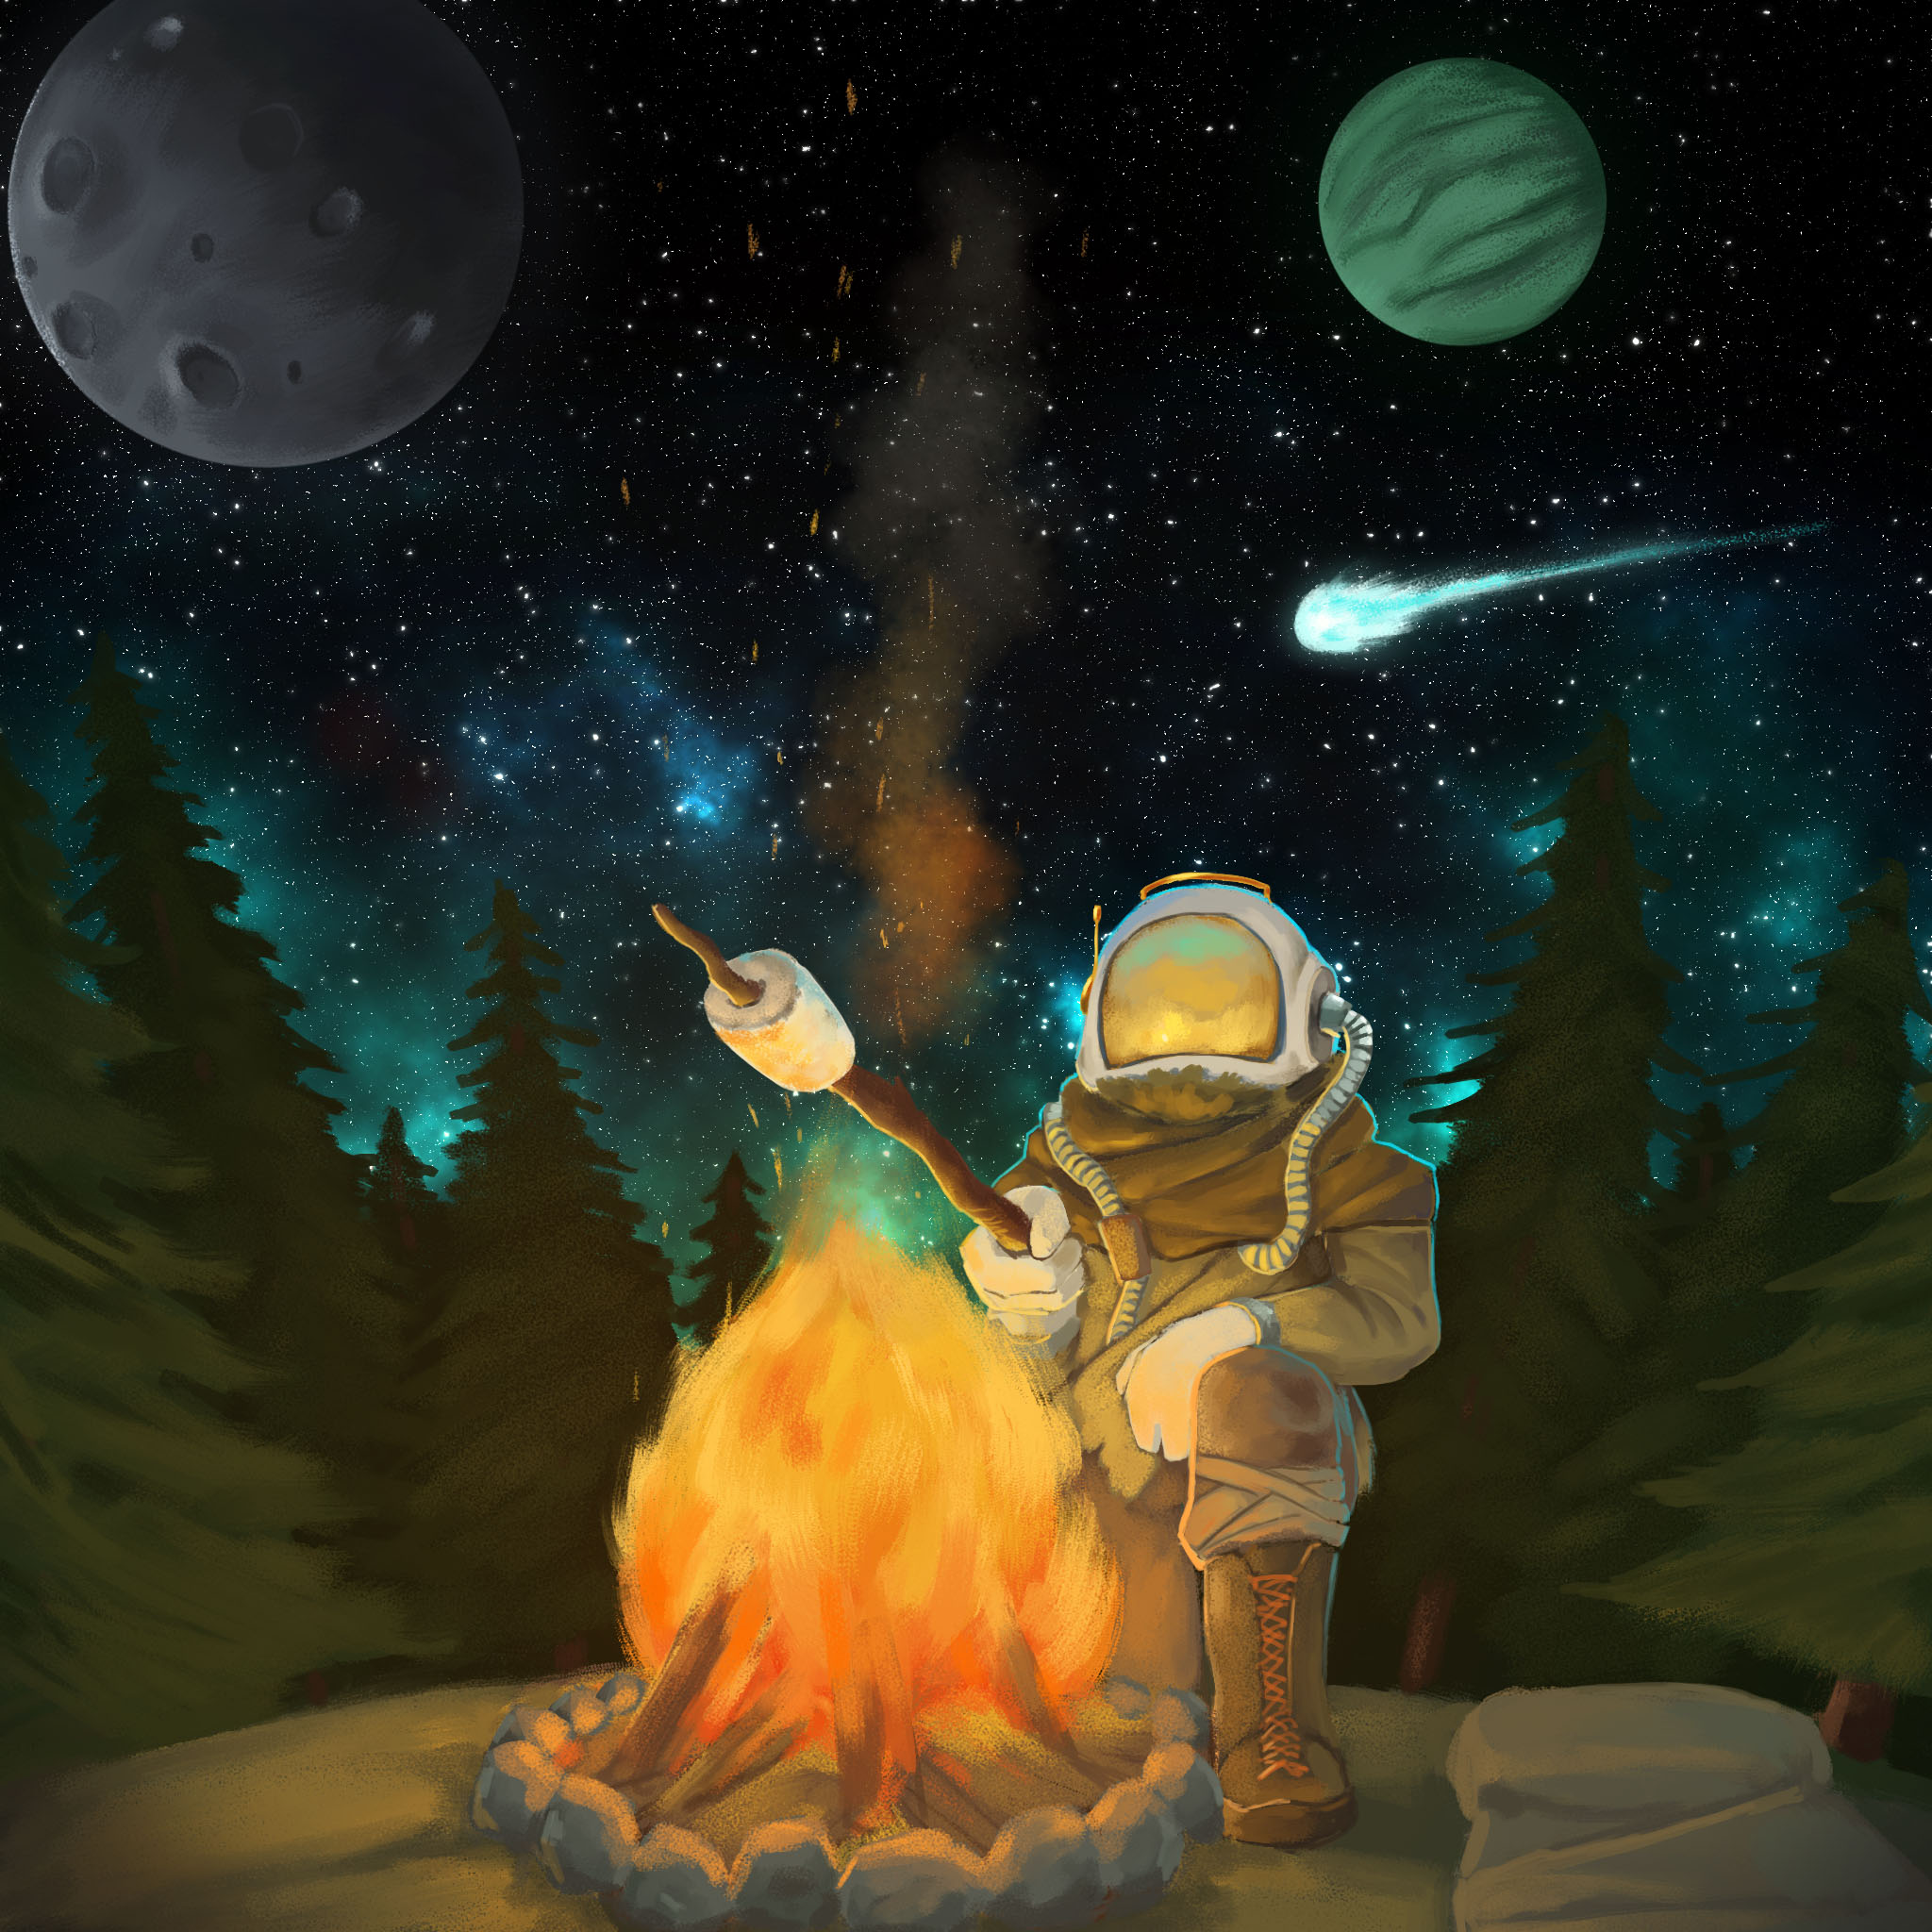
\includegraphics[scale=0.09]{imagenes/outer wilds.jpeg}
        \caption{Outer Wilds.}
        \label{fig:outer wilds}
    \end{center}
\end{figure}

\begin{wrapfigure}{r}{0.4\textwidth}
  \begin{center}
    
\includegraphics[width=0.25\textwidth]{imagenes/balatro.pdf}
  \caption{Balatro.}
  \end{center}
\end{wrapfigure}

También se pueden configurar imágenes alrededor del texto con \verb|wrapfigure| del paquete \verb|wrapfig|. Más info \href{https://www.overleaf.com/learn/latex/Wrapping_text_around_figures}{acá}. Generemos un poco de texto para ver cómo se acomoda.

\lipsum[1] % Generamos un párrafo de texto relleno]

\subsection{Tablas}

Las \textbf{tablas} se crean con el comando \verb|tabular|. Hay muchísimo para personalizar, más info sobre eso \href{https://www.overleaf.com/learn/latex/Tables}{acá}.
\begin{center}
    \begin{tabular}{ ||c|c|c|| } 
     \hline
     Nombre & Apellido & Categoría \\ 
     \hline
     Harry & Potter & Monotributista \\ 
     Luke & Skywalker & Responsable Inscripto \\ 
     \hline
    \end{tabular}
\end{center}
También se pueden crear tablas automáticamente de archivos \verb|.csv| con el paquete \verb|csvsimple|:

\begin{center}
    \csvautotabular{data/medialunas.csv}
\end{center}

\subsection{Gráficos y diagramas}

La librería \verb|tikz| va a ser tu mejor amigo. Se pueden hacer desde diagramas conmutativos hasta grafos y gráficos de funciones, entre otras cosas. Una cosa a tener en cuenta es que \LaTeX\ no está hecho para generar gráficos excesivamente pesados (y además los de Overleaf son bastante amarretes con el tiempo de compilación permitido). Si querés graficar muchas cosas o cosas bastante pesadas para el compilador, considerá usar \LaTeX\ offline y/o importar los gráficos de otro software.

Algunos ejemplos concretos:
\begin{itemize}
    \item \textit{Gráficos} de funciones y curvas con el paquete \verb|pgfplots|: ver
    \[
        \verb|articulo_solo_graficos.tex|
    \]
    \item \textit{Grafos}. Hay una infinidad de formas de hacer grafos conocidos y personalizarlos. Más info en \url{https://tikz.dev/tikz-graphs}.

\begin{center}
    %  Configuramos los nodos de la forma que queremos
    \tikz \graph [empty nodes, nodes={circle, draw, inner sep=0.05cm,fill}] {
        %  Creamos los vértices y aristas
        a[label=$a$] -- {b[label=$b$], c[label=$c$]} <- f[label=$f$];
        % Al especificar la label, se puede poner un prefijo indicando donde ubicarla. Por ejemplo "right:$d$" ubica la label "d" a la derecha del vértice
        e[label=$e$] -> d[label=right:$d$];
        d -- c;
    };
\end{center}
Una forma un poco más manual pero que permite control sobre las posiciones de los vértices es la siguiente:
\begin{center}
 \begin{tikzpicture}
    \node (x) at (0,0) [label=below left:$a$,point];
    \node (y) at (2,0) [label=below right:$b$,point];
    \node (z) at (1,1.5) [label=above:$c$,point];
    \node (w) at (3,1.5) [label=above:$d$,point];
    \draw (x) -- (y) -- (z) -- (x);
    \draw (y) -> (w);
\end{tikzpicture}
\end{center}

\item \textit{Diagramas conmutativos:}

\[
    \begin{tikzcd}
        % Luego de cada "nodo" del diagrama van comandos \arrow especificando en qué dirección va la flecha y qué etiqueta tiene
        X \arrow[r, "T"] \arrow[d, "J"] & X \arrow[d, "J"] \\
         X_0 \arrow[r, "T_0"] & X_0
    \end{tikzcd}\hspace{1.5cm}
    \begin{tikzcd}
        & X \arrow[d, dashed, "\exists ! f"] \arrow[ld, "f_1"'] \arrow[rd, "f_2"] & \\
        A & A \times B \arrow[l, "\pi_1"] \arrow[r, "\pi_2", swap]  & B
    \end{tikzcd}
\]
\item Otros gráficos varios. Tomátelo con calma, empezá a dibujar formas y cambiar los valores para ver cómo te va quedando. No es trabajo digno.

  \begin{center}
    \begin{tikzpicture}[scale=0.8]
      % Definimos algunos estilos
      \tikzstyle{var_dif_center}=[
        circle,
        fill=black,
        inner sep=0pt,
        minimum width=0.15cm
      ]
      % contorno de la variedad
      % "smooth cycle, tension=.7" hace que las coordenadas especificadas se unan como curvas y no poligonalmente
      \tikzstyle{var_dif}=[smooth cycle, tension=.7]
      % espacio euclideo
      \tikzstyle{esp_euc}=[smooth cycle, tension=1]
      % un entorno dentro de la variedad
      \tikzstyle{entorno}=[
          circle,
          minimum size =1.3cm,
          dashed,
          draw=black
      ]

      % M^d
      \draw[var_dif] plot coordinates{ (0,0) (0.75,1.75) (2.5,2) (3,0)};
      \node[var_dif_center, label={above, yshift=0cm, xshift=0cm, scale=0.8: $m$}] (Mcenter) at (1.5, 0.8) {};
      \node (M) at (0.35, 0.35) {$M$};
      \node[entorno, label={above, yshift=-1.1cm, xshift=-.34cm, scale=0.75: $\tilde{U}$}] (U) at (1.5, 0.8) {};

      % N^c
      \draw[var_dif] plot coordinates{ (0 + 6,0) (0.75 + 6,1.75) (2.5 + 6,2) (3 + 6,0) };
      \node[var_dif_center, label={above, yshift=0cm, xshift=0cm, scale=0.72: $f(m)$}] (Ncenter) at (1.5 + 6, 0.8) {};
      \node (N) at (0.35 + 6, 0.35) {$N$};
      \node[entorno, label={above, yshift=-1.1cm, xshift=.4cm, scale=0.75: $V$}] (V) at (1.5 + 6, 0.8) {};

      % R^d
      \draw[esp_euc] plot coordinates{ (0, -4.2) (1.5,1.5 - 4.2) (3,0 - 4.2) (1.5, -1.5 - 4.2) };
      \node (Rd) at (0.9, -3.5) {$\real^d$};
      \node[var_dif_center, label={below, yshift=0cm, xshift=-0.25cm, scale=0.85: $\varphi(m)$}] (Rdcenter) at (1.5, -4.4) {};

      % R^d 2
      \draw[esp_euc] plot coordinates{ (0 + 6, -4.2) (1.5 + 6, 1.5 - 4.2) (3 + 6, 0 - 4.2) (1.5 + 6, -1.5 - 4.2) };
      \node (Rc) at (0.9 + 6, -3.5) {$\real^d$};
      \node[var_dif_center, label={below, yshift=0cm, xshift=-0cm, scale=0.8: $\psi(f(m))$}] (Rd2center) at (1.5 + 6, -4.4) {};

      % phi
      \draw (Mcenter) edge[->, out=-80,in=80, shorten <= 0.1cm, shorten >= 0.1cm] node[auto] {$\varphi$} (Rdcenter);
      
      % psi
      \draw (Ncenter) edge[->, out=-80,in=80, shorten <= 0.1cm, shorten >= 0.1cm] node[auto] {$\psi$} (Rd2center);
      
      % f
      \draw (Mcenter) edge[->, out=10,in=170, shorten <= 0.1cm, shorten >= 0.1cm] node[auto, label={above, yshift=-0.2cm, scale=1:$f$}] {} (Ncenter);

      % psi o f o phi^(-1)
      \draw (Rdcenter) edge[->, dashed, out=10,in=170, shorten <= 0.1cm, shorten >= 0.1cm] node[auto, label={above, yshift=-0.2cm, scale=1:$F$}] {} (Rd2center);
    \end{tikzpicture}
    \vspace{.1cm}
  \end{center}


\end{itemize}








\end{document}